\section{Dataset Size and \texorpdfstring{$\theta_{pos}$}{theta\_pos}}
\label{sec:pos-harmony-size}

$KL_{cpos^{3}}(tgt, src)$ is defined on distributions of trigrams found in $tgt$ and $src$. The calculated metric scores should therefore be affected by the presence or absence of the POS trigrams. The presence/absence of POS trigrams can similarly affect the calculations of $\theta_{pos}$ metric scores. In this part of the experiment, we use k-fold cross validation to check the effect of presence/absence of POS trigrams in the data. We use k-fold cross validation here as it allows us to check how the calculated scores are affected based on the size of the data alone, and also to frame an association of the scores with the presence/absence of POS trigrams, if any. 

The presence/absence of data from different genres can affect the calculation of $\theta_{pos}$ scores. In order to discount such effect, the entire data used for the analysis should belong to the same genre. For this experiment, we used \verb|cs|-PDT (rated 4.5/5 stars) and \verb|et|-EDT (rated 4/5 stars) treebanks. The motivation behind the selection of languages is primarily the difference in their language families. Additionally, the two treebanks contain a large number of sentences belonging to the \textit{news} genre, making it easier for the data to be studied across multiple k-fold runs with different k-values. Table \ref{tab:pos-harmony-size-datasize} lists the sentences counts associated to the considered genres in either treebank.

\begin{table}[H]
    \centering
    \begin{tabular}{|c|l|l|}
        \hline
        \textbf{Language} & \textbf{Genre} & \textbf{Sentences}\\
        \hline
        \texttt{cs} & News & 53 075 \\
        \hline
        \texttt{et} & News & 13 557 \\
        \hline
    \end{tabular}
    \caption{Sentence Counts in \texttt{cs}-PDT and \texttt{et}-EDT Treebanks}
    \label{tab:pos-harmony-size-datasize}
\end{table}


To check the effect of data size on $\theta_{pos}$ metric, we ran k-fold cross validation on the data from the aforementioned treebank in the following manner:

\begin{enumerate}
    \item Concatenate the different splits of the treebank together before downsampling the concatenated data to a fixed number of instances.
    \item For different predetermined k-values, the downsampled data is split into k folds. In each fold, the $\theta_{pos}$ scores are calculated between the fold's splits.
    \item In each fold, we try to estimate the projection of trigram distribution from the test set for the fold, onto the training set for the fold. Essentially, the training set in a fold corresponds to $src$, while the test set corresponds to $tgt$. We try to calculate coverage of different POS trigrams in each fold. The coverage is calculated by counting the number of trigrams common to both $src$ and $tgt$, expressed as a percentage of the total number of trigrams in $tgt$.
\end{enumerate}

The methodology as stated above is listed for a single repetition over a single treebank. To get a better estimation of the values, the method was repeated 100 times each for both the treebanks. In each repetition, the seed values were uniquely selected so as to get different downsamples every time. Table \ref{tab:pos-harmony-size} lists the number of instances the treebank was downsampled to, and the considered k values for the downsampled data. The table also lists the $\theta_{pos}$ scores and coverage scores for each fold. The scores are averaged over the 100 repetitions for each k-value, with the standard deviation (sd) also mentioned therein.

\begin{table}[H]
    \centering
    \begin{tabular}{|c|c||c|l|l|}
        \hline
        \textbf{Language} & \textbf{Downsample} & \textbf{k value} & \textbf{$\theta_{pos}$ Score} & \textbf{Coverage (in \%)}\\
        \hline
        \hline
        \multirow{7}{*}{\texttt{cs}} & \multirow{7}{*}{50000} & 5 & 0.021 $\pm$ 0.001 & 83.904 $\pm$ 0.563\\
        & & 10 & 0.037 $\pm$ 0.001 & 75.457 $\pm$ 0.602\\
        & & 20 & 0.069 $\pm$ 0.002 & 66.138 $\pm$ 0.656\\
        & & 50 & 0.161 $\pm$ 0.005 & 52.754 $\pm$ 0.832\\
        & & 100 & 0.304 $\pm$ 0.011 & 42.368 $\pm$ 0.843\\
        & & 250 & 0.663 $\pm$ 0.03 & 29.353 $\pm$ 0.864\\
        & & 500 & 1.092 $\pm$ 0.063 & 20.802 $\pm$ 1.021\\
        \hline
        \hline
        \multirow{8}{*}{\texttt{et}} & \multirow{8}{*}{12000} & 4 & 0.064 $\pm$ 0.002 & 76.15 $\pm$ 0.807\\
        & & 6 & 0.087 $\pm$ 0.003 & 69.739 $\pm$ 0.957\\
        & & 8 & 0.109 $\pm$ 0.004 & 65.237 $\pm$ 0.83\\
        & & 12 & 0.155 $\pm$ 0.006 & 58.667 $\pm$ 1.032\\
        & & 16 & 0.2 $\pm$ 0.007 & 54.124 $\pm$ 1.029\\
        & & 24 & 0.286 $\pm$ 0.012 & 47.77 $\pm$ 1.046\\
        & & 48 & 0.52 $\pm$ 0.02 & 37.096 $\pm$ 0.947\\
        & & 120 & 1.038 $\pm$ 0.053 & 24.485 $\pm$ 1.151\\
        \hline
    \end{tabular}
    \caption[$\theta_{pos}$ and Coverage of POS Trigram Scores ($\pm$ sd) Averaged over 100 Different Runs to Highlight the Effect of Size Disparity]{$\theta_{pos}$ and Coverage of POS Trigram Scores ($\pm$ sd) Averaged over 100 Different Runs to Highlight the Effect of Size Disparity. The values in the $\theta_{pos}$ and Coverage columns are the representative scores for the k-value, selected from the scores of individual runs such that the score is statistically equal to scores of more than 50\% of the runs in the fold. The statistical value is calculated at 95\% confidence using One Sampled t-test.}
    \label{tab:pos-harmony-size}
\end{table}

Looking at the scores for the two languages, there is a clear negative correlation between coverage and $\theta_{pos}$ score. Coverage of different POS trigrams is, however, dependent upon the size of the datasets being compared. In case of a really small dataset, the number of different POS trigrams or even the total number of POS trigrams is not comparable.

Figures \ref{fig:trigram-PDT} and \ref{fig:trigram-EDT} consist of two graphs each. The graphs show how the number of (i) distinct POS trigrams, and (ii) total number of POS trigrams is affected by a change in the dataset size. While the first graph in each figure shows the variability across the entire downsampled data (50000 sentences in \texttt{cs} in Figure \ref{fig:trigram-PDT}, and 12000 sentences in \texttt{et} in Figure \ref{fig:trigram-EDT}); the second graph zooms in on the progression over 2000 sentences.

\begin{figure}[H]
    \centering
    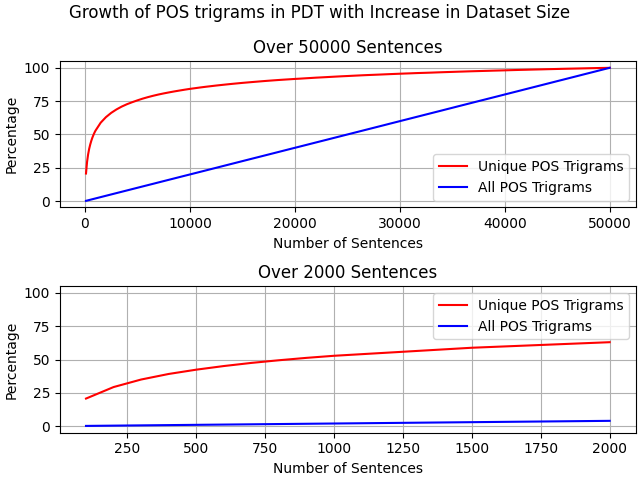
\includegraphics[scale=0.75]{img/trigram-stats-PDT.png}
    \caption{Growth of POS Trigrams in PDT with Increase in Dataset Size}
    \label{fig:trigram-PDT}
\end{figure}

\begin{figure}[H]
    \centering
    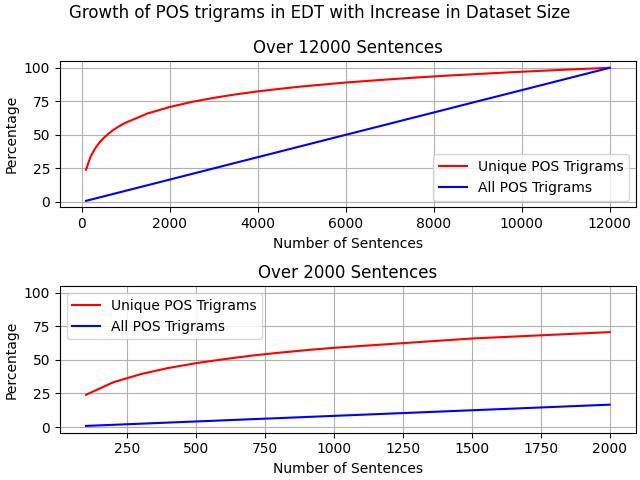
\includegraphics[scale=0.75]{img/trigram-stats-EDT.png}
    \caption{Growth of POS Trigrams in EDT with Increase in Dataset Size}
    \label{fig:trigram-EDT}
\end{figure}

As can be seen from the figures, the growth pattern is similar across both the languages. We can see that in case of a considerably small dataset size, the POS trigrams can not be considered as representative of those present in the entire dataset. We claim that for a proper estimation of the annotation consistency in two datasets belonging to the same genre, either dataset requires at least 400 sentences ($\approx 40\%$ of unique POS trigrams) for the estimation to be reliable. The minimum limitation on the size of the datasets ensures that the distribution of POS trigrams in either dataset is not skewed because of a small size.

\begin{claim}
Data in a given genre can be compared across two datasets $A, B$ iff \\
\begin{equation*}
    \boxed{size(A) \geq 400 \And size(B) \geq 400}
\end{equation*}
\label{claim:pos_size_init}
\end{claim}

where $size(X)$ refers to the size of dataset $X$ in terms of the number of sentences

Table \ref{tab:counts-ar} shows the average sentence length of sentences in different treebanks for \verb|ar|. If we consider equal number of sentences from either of \verb|ar|-NYUAD or \verb|ar|-PADT treebanks and compare the POS annotation consistency with \verb|ar|-PUD treebanks, the total number of syntactic words differ by a factor of almost 2. 

\begin{table}[H]
    \centering
    \begin{tabular}{|l|l|l|l|}
    \hline
    \textbf{Counts} & \texttt{ar}-NYUAD & \texttt{ar}-PADT & \texttt{ar}-PUD \\
    \hline
    Syntactic Words & 738889 & 282384 & 20751 \\
    Sentences & 19738 & 7664 & 1000\\
    \hline
    \textbf{Average} & 37.434 & 36.845 & 20.751\\
    \hline
    \end{tabular}
    \caption[Average Sentence Lengths in \texttt{ar} Treebanks]{Average Sentence Lengths in \texttt{ar} Treebanks. In \texttt{es}, the token \textbf{v\'amonos} (Let's go) is split into 2 syntactic words \textbf{vamos} (go-\textit{1P-Pl.}) and \textbf{nos} (\textit{1P.-Pl.}) for annotation.}
    \label{tab:counts-ar}
\end{table}

When calculating the $\theta_{pos}$ scores for a set of treebanks, the average sentence length in either treebank should also be taken into account. It makes sense to limit the size of the datasets in consideration not in absolute terms, but also in reference to each other. Keeping this in mind, we update Claim \ref{claim:pos_size_init} to account for the average sentence length in Claim \ref{claim:pos_size}.

\begin{claim}
Data in a given genre can be compared across two datasets $A, B$ iff \\
\begin{equation}
\label{eqn:size_constraint}
    \boxed{size(A) \geq 400 \And Avg(A) \geq Avg(B) \implies size(B) \geq Avg(A) \cdot 400}
\end{equation}
\label{claim:pos_size}
\end{claim}

where 
\begin{enumerate}
    \item $Avg(X) = \frac{Total Syntactic Words(X)}{size(X)}$ is the average sentence length in dataset $X$
    \item $size(X)$ refers to the size of dataset $X$ in terms of the number of sentences
\end{enumerate}

From the results of the data in Table \ref{tab:pos-harmony-size}, when the test split is composed of 500 instances ($k=100$ for \texttt{cs}; $k=24$ for \texttt{et}), the $\theta_{pos}$ metric is $\approx 0.3$. Considering that the larger $k$-values in either dataset do not satisfy the condition in Equation \ref{eqn:size_constraint}, we use the values as per the aforementioned $k$-values to estimate the maximal value for $\theta_{pos}$ when there is a size variance in the datasets.

As mentioned earlier, the treebanks in the consideration are ranked high in their quality check. Considering that some treebanks might not have such high quality of annotation, we allow some room for the change in $\theta_{pos}$ metric. We can set up the limit on the $\theta_{pos}$ metric with respect to dataset size change as in Equation \ref{eqn:theta_pos_size_limit}, with datasets $A$, $B$ containing data from same genre, and subjected to condition as in Equation \ref{eqn:size_constraint}.

\begin{equation}
    \boxed{\theta_{pos}(A,B) \leq \Theta_{pos}(A,B) = 0.5}
\label{eqn:theta_pos_size_limit}
\end{equation}

\newpage